\chapter{Software}
In wat volgt, wordt het ontwerpproces van de software uitvoerig besproken en wordt een verantwoording gegeven van de ontwerpskeuzes.

\section{Verbinding tussen de UWB location anchors en tag} \label{sec:uwb_tag}
Ultra Wide Band (UWB) \cite{uwb2016}.\\

Een belangrijk aspect naast nauwkeurigheid, is de snelheid.
We zullen dus ook een algoritme moeten schrijven die bepaalt op welke ankers hij zich basseert.
Het zou een beetje over-kill zijn als hij alle ankers in het volledige magazijn aanspreekt voor zijn locatie.
Een mogelijke manier zou zijn dat we op voorhand bepalen dat hij gebruik maakt van het anker waar hij zich het dichtst bij bevindt en 4 ankers die zich in de buurt bevinden.\\

Nog een element die we in rekening moeten brengen is dat de server mogelijks enkel 2D ondersteunt, wat dus niet voldoet voor een drone die op verschillende hoogtes kan vliegen.
Gelukkig zit er in de drone een ultrasone sensor en een barometer ingebouwd die zijn hoogte kan bepalen.

\section{Verbinding tussen de Raspberry Pi Zero W en de server} \label{sec:raspberry_server}
Wanneer de controller afstanden ontvangt tot gekende ankers, moeten deze nog verwerkt worden tot de correcte locatie binnen de ruimte.
Hiervoor kunnen we gebruik maken van een Mosquitto server die deze complexe berekeningen op zich neemt.
Communicatie met de Mosquitto server werkt via het MQTT protocol.\\

\section{Verbinding tussen de server en de Raspberry Pi 3 B} \label{sec:server_raspberry}
De off-board controller zal via dat zelfde MQTT protocol posities van de drone en van de waypoints van de server verkrijgen.
Op deze plaats wordt dan een algoritme uitgevoerd dat de aansturingsinstructies voor de drone zal bepalen en uiteindelijk ook versturen.\\

Hier hebben we 2 algoritmes voor geschreven:\\
In het eerste algoritme zal de drone enkel draaien rond de z-as en voorwaarts bewegen als hij in de juiste richting kijkt.
Natuurlijk kan de drone nog steeds op en neer bewegen langs de z-as, onafhankelijk van de bewegingen in het xy-vlak.
Eerst draaien en dan pas zich naar voor verplaatsen is een vrij trage manier om in een kamer te bewegen.
Deze bewegingen kunnen niet tegelijk gebeuren of de drone wijkt al snel af van z'n oorsponkelijk pad.\\
In een tweede algoritme zal de drone nooit draaien.
Hij zal enkel naar voor, achter, links rechts, op een neer bewegen.
Uiteraard worden ook kleine correcties aangebracht om de voorkant van de drone steeds in de juiste richting te doen wijzen.
Deze methode is een hoop sneller, omdat er meer richtingen zijn waarin de drone zich kan voortbewegen.\\

Bij beide algoritmes probeert de drone om een reeks targets \'e\'en voor \'e\'en te bezoeken, eerder dan een bepaald traject binnen een bepaalde tijd af te leggen.
Pas zodra een target bezocht is, gaat de drone naar de volgende plek.
Er worden dus geen waypoints over geslaan als de drone achter raakt op schema.\\
In de praktijk kunnen deze waypoints overeenkomen met dozen die gescand moeten worden.\\
Dit betekent ook dat collision detection tussen mogelijks kruisende drones ook live dient te gebeuren, om te voorkomen dat drones die voor of achter of schema zijn tegen elkaar vliegen.

\section{Verbinding tussen de Raspberry Pi 3 B en de drone} \label{sec:raspberry_drone}
De drone zet een eigen wifi-netwerk met ESSID adrone2\_XXXXXX  op en geeft zichzelf vaak het IP-adres 192.168.1.1.
Als de Raspberry Pi 3 B verbindt met het netwerk van de drone, krijgt het een IP-adres tussen 192.168.1.2 en 192.168.1.5 (met de grenzen inbegrepen) toegekend.
Indien de drone een ander IP-adres aan zichzelf toegekend heeft, zullen de gebruikers één van de 4 volgende adressen toegekend krijgen.\\
Het besturen van de drone gebeurd door het versturen van \textit{AT commands} op UDP poort 5556.
De maximale frequentie waarmee de commando's kunnen doorgestuurd worden ligt rond de \SI{30}{\Hz}, om de drone snel te kunnen laten reageren, en een goede gebruikerservaring te garanderen.\\

Informatie over de drone (zoals status, positie, snelheid, snelheid van de rotoren, ...) wordt naar de gebruiker gestuurd op UDP poort 5554.
De frequentie waarmee deze \textit{navdata} wordt verstuurd ligt tussen de \SI{15}{\Hz} (in demo mode) en \SI{200}{\Hz} in full (debug) mode.\\
Om belangrijke data, zoals informatie voor de configuratie, te versturen maakt men geen gebruik van UDP, maar van TCP.
Dit gebeurd via de \textit{control port} 5559. \cite{developer_guide2012}\\
De AT commands en navdata worden gestuurd en ontvangen a.d.h.v. een library.

\section{Setup} \label{sec:setup_software}
Op figuur \ref{fig:setup_software} vindt u de hardware setup, aangevuld met protocollen.
\begin{figure}[p]
	\centering
	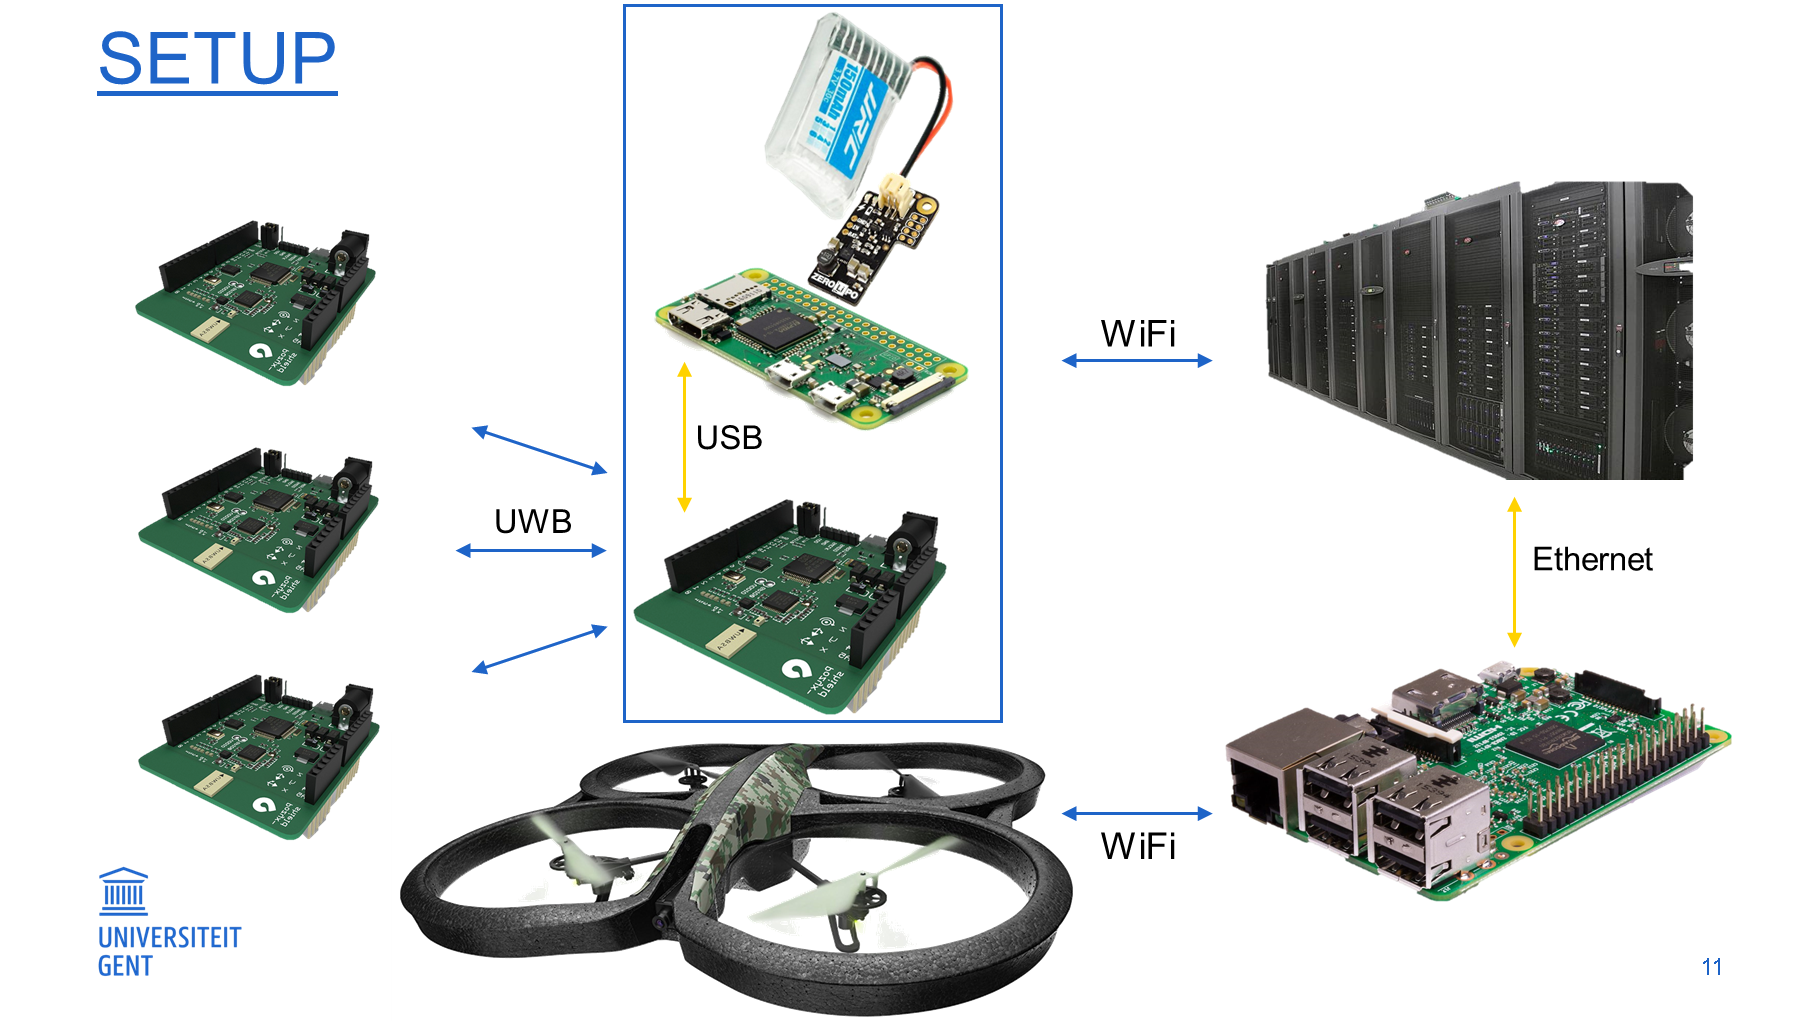
\includegraphics[width=\textwidth]{Setup}
	\caption[Hardware setup, aangevuld met protocollen]{Hardware setup, aangevuld met protocollen.}
	\label{fig:setup_software}
\end{figure}

\section{Visualisatie} \label{sec:visualization}
